\documentclass{article}
\usepackage[utf8]{inputenc}
\usepackage{listings}
\usepackage{multimedia} % to embed movies in the PDF file
\usepackage{graphicx}
\usepackage{comment}
\usepackage[english]{babel}
\usepackage{amsmath}
\usepackage{amsfonts}
\usepackage{subfigure}
\usepackage{wrapfig}
\usepackage{multirow}
\usepackage{tikz}
\usepackage{verbatim}
\usepackage{float}
%!TEX root = main.tex



\newcommand{\eref}[1]{\mbox{\rm(\ref{#1})}}
\newcommand{\tref}[1]{\mbox{\rm\ref{#1}}}
\newcommand{\set}[2]{\left\{ #1 \; : \; #2 \right\} }
\newcommand{\deq}{\raisebox{0pt}[1ex][0pt]{$\stackrel{\scriptscriptstyle{\rm def}}{{}={}}$}}

\newcommand {\DS} {\displaystyle}

\newcommand{\real}{\mathbb{R}}



\newcommand {\half} {\mbox{$\frac{1}{2}$}}
\newcommand{\force}{{\mathbf{f}}}
\newcommand{\strain}{{\boldsymbol{\varepsilon}}}
\newcommand{\stress}{{\boldsymbol{\sigma}}}
\renewcommand{\div}{{\boldsymbol{\nabla}}}

\newcommand {\cA} {{\cal A}}
\newcommand {\cB} {{\cal B}}
\newcommand {\cC} {{\cal C}}
\newcommand {\cD} {{\cal D}}
\newcommand {\cE} {{\cal E}}
\newcommand {\cK} {{\cal K}}
\newcommand {\cL} {{\cal L}}
\newcommand {\cP} {{\cal P}}
\newcommand {\cQ} {{\cal Q}}
\newcommand {\cR} {{\cal R}}
\newcommand {\cV} {{\cal V}}
\newcommand {\cW} {{\cal W}}
\newcommand {\CC} {{\cal C}}
\newcommand {\CD} {{\cal D}}
\newcommand {\CH} {{\cal H}}
\newcommand {\CS} {{\cal S}}
\newcommand {\CU} {{\cal U}}
\newcommand {\CY} {{\cal Y}}



\newcommand{\bzero}{\mathbf{0}}
\newcommand{\ba}{\mathbf{a}}
\newcommand{\bb}{\mathbf{b}}
\newcommand{\bc}{\mathbf{c}}
\newcommand{\bd}{\mathbf{d}}
\newcommand{\be}{\mathbf{e}}
\newcommand{\bg}{\mathbf{g}}
\newcommand{\bh}{\mathbf{h}}
\newcommand{\bl}{\mathbf{l}}
\newcommand{\bn}{\mathbf{n}}
\newcommand{\bp}{\mathbf{p}}
\newcommand{\bq}{\mathbf{q}}
\newcommand{\br}{\mathbf{r}}
\newcommand{\bs}{\mathbf{s}}
\newcommand{\bt}{\mathbf{t}}
\newcommand{\bu}{\mathbf{u}}
\newcommand{\bv}{\mathbf{v}}
\newcommand{\bw}{\mathbf{w}}
\newcommand{\bx}{\mathbf{x}}
\newcommand{\by}{\mathbf{y}}
\newcommand{\bz}{\mathbf{z}}
\newcommand{\bA}{{\mathbf A}}
\newcommand{\bB}{\mathbf{B}}
\newcommand{\bC}{\mathbf{C}}
\newcommand{\bD}{\mathbf{D}}
\newcommand{\bE}{\mathbf{E}}
\newcommand{\bF}{\mathbf{F}}
\newcommand{\bG}{\mathbf{G}}
\newcommand{\bH}{\mathbf{H}}
\newcommand{\bI}{\mathbf{I}}
\newcommand{\bJ}{\mathbf{J}}
\newcommand{\bK}{\mathbf{K}}
\newcommand{\bL}{\mathbf{L}}
\newcommand{\bM}{\mathbf{M}}
\newcommand{\bN}{\mathbf{N}}
\newcommand{\bO}{\mathbf{O}}
\newcommand{\bP}{\mathbf{P}}
\newcommand{\bQ}{\mathbf{Q}}
\newcommand{\bR}{\mathbf{R}}
\newcommand{\bS}{\mathbf{S}}
\newcommand{\bU}{\mathbf{U}}
\newcommand{\bV}{\mathbf{V}}
\newcommand{\bW}{\mathbf{W}}
\newcommand{\bX}{\mathbf{X}}
\newcommand{\bY}{\mathbf{Y}}
\newcommand{\bZ}{\mathbf{Z}}

\newcommand{\bgamma}{{\boldsymbol{\gamma}}}
\newcommand{\bmu}{{\boldsymbol{\mu}}}
\newcommand{\bkappa}{{\boldsymbol{\kappa}}}
\newcommand{\blambda}{{\boldsymbol{\lambda}}}
\newcommand{\bLambda}{{\boldsymbol{\Lambda}}}
\newcommand{\bpi}{{\boldsymbol{\pi}}}
\newcommand{\bPi}{{\boldsymbol{\Pi}}}
\newcommand{\btheta}{{\boldsymbol{\theta}}}
\newcommand{\bTheta}{{\boldsymbol{\Theta}}}
\newcommand{\bSigma}{{\boldsymbol{\Sigma}}}






\title{AMATH 585 Homework 2}
\author{Cade Ballew}
\date{January 24, 2022}

\begin{document}

\maketitle

\section{Problem 1}
\subsection{Part a}
If we consider the BVP
\[
\frac{d}{dx} \left( c(x) \frac{du}{dx} \right) = f(x) ,~~~
0 \leq x \leq 1 ,
\]
\[
u(0) = 1,~~~u'(1) = 0,
\]
the method of differencing discussed in class and given at (2.72) in the text gives that
\[
(cu')(x_i)\approx\frac{1}{h^2}(c_{i-1/2}u_{i-1}-(c_{i-1/2}+c_{i+1/2})u_i+c_{i+1/2}u_{i+1})
\]
if we consider the standard grid $0=x_0<x_1<\ldots<x_m<x_{m+1}=1$ with spacing $h$. We will consider this for $i=1,\ldots, m+1$ To deal with the endpoints, we use the second approach for dealing with Neumann boundary conditions described in section 2.12 of the text. We first handle the Dirchlet condition in the standard way by taking $u_0=1$ and substituting this into our equation for $i=1$ to get that 
\[
f(x_1)=\frac{1}{h^2}(c_{1/2}-(c_{1/2}+c_{3/2})u_1+c_{3/2}u_{2})
\]
so 
\[
\frac{1}{h^2}(-(c_{1/2}+c_{3/2})u_1+c_{3/2}u_{2})=f(x_1)-\frac{1}{h^2}c_{1/2}
\]
Now, we introduce a ghost point $u_{m+2}$ and apply a centered difference approximation to $u'(1)$. Namely,
\[
0=u'(1)\approx\frac{1}{2h}(x_{m+2}-x_m)
\]
and solve to get that $x_{m+2}=x_m$. Now, we apply this to the above difference equation at $i=m+1$ to get 
\begin{align*}
f(x_{m+1})&=\frac{1}{h^2}(c_{m+1/2}u_{m}-(c_{m+1/2}+c_{m+3/2})u_{m+1}+c_{m+3/2}u_{m+2})\\&=\frac{1}{h^2}((c_{m+1/2}+c_{m+3/2})u_{m}-(c_{m+1/2}+c_{m+3/2})u_{m+1}).
\end{align*}
Now, we consider $c(x)=1+x^2$ and plug this into our equations. First, note that 
\[
c_{i-1/2}+c_{i+1/2}=1+(x_i-h/2)^2+1+(x_i+h/2)^2=2(1+x_i^2+(h/2)^2).
\]
For $i=0$, we simply have that 
\[
u_0=1,
\]
but we have already substituted this into our remaining equations. For $i=1$, 
\begin{align*}
&\frac{1}{h^2}(-2(1+x_1^2+(h/2)^2)u_1+(1+(x_1+h/2)^2)u_{2}=f(x_1)-\frac{1}{h^2}(1+(x_1-h/2)^2).
\end{align*}
For $i=2,\ldots m$,
\[
\frac{1}{h^2}((1+(x_i-h/2)^2)u_{i-1}-2(1+x_i^2+(h/2)^2)u_i+(1+(x_i+h/2)^2)u_{i+1})=f(x_i).
\]
For $i=m+1$,
\[
\frac{1}{h^2}(2(1+x_{m+1}^2+(h/2)^2)u_{m}-2(1+x_{m+1}^2+(h/2)^2)u_{m+1})=f(x_{m+1}).
\]
Note that this yields $m+1$ equations and $m+1$ unknowns if we ignore the $i=0$ case.

\subsection{Part b}
To implement this in MATLAB, we take $u(x) = (1-x )^2$ which gives $f(x) = 2( 3 x^2 - 2 x + 1 )$. We do not implement the $i=0$ equation since we have already substituted $u_0=1$ into our other equations (though primarily to remain consistent with MATLAB's oft-annoying index convention). \\
The following MATLAB function takes as inputs function handles for $c(x)$, $u(x)$, and $f(x)$ as well as $m$ and outputs the computed solution vector $u$, the stepsize $h$, and a vector of errors at each gridpoint. 
\begin{verbatim}
function [u,h,errvec] = rodFD(c,utrue,ftrue,m)
h=1/(m+1);
x = linspace(0,1,m+2)';
x = x(2:end); %remove x_0=0 fo indexing

A=zeros(m+1);
A(1,1:2)=[-(c(x(1)-h/2)+c(x(1)+h/2)), c(x(1)+h/2)]/h^2; %equation i=1
A(m+1,m:m+1)=[c(x(m+1)-h/2)+c(x(m+1)+h/2), -(c(x(m+1)-h/2)+c(x(m+1)+h/2))]/h^2; %i=m+1
for i = 2:m %interior
    A(i,i-1:i+1)=[c(x(i)-h/2), -(c(x(i)-h/2)+c(x(i)+h/2)), c(x(i)+h/2)]/h^2;
end

f = ftrue(x);
f(1)=f(1)-c(x(1)-h/2)/h^2; %Dirichlet BC

u=A\f;
u=[1;u]; %append u_0=1 to solution vector
x = [0;x]; %reappend x_0=0
uexact=utrue(x);
errvec=u-uexact;
end
\end{verbatim}

\subsection{Part c}
We call this function for the $c,u,f$ stated above and for $m=9,99,999,9999$ (after running into memory issues with $m=99999$) which corresponds to $h=0.1,0.01,0.001,0.0001$ using the following code which also computes the error in the infinity norm.
\begin{verbatim}
for m=[9,99,999,9999]
    [u,h,errvec]=rodFD(c,utrue,ftrue,m);
    errinf=norm(errvec,'inf');
    fprintf('%.e       %e\n',h,errinf)
end
\end{verbatim}
The following table gives the computed error at our chosen values of h.
\begin{table}[H]\centering
\begin{tabular}{|r|r|} \hline
{h}&{Infinity norm error}\\\hline
1e-01&       2.183269e-03\\
1e-02&       2.194014e-05\\
1e-03&       2.194123e-07\\
1e-04&       2.125117e-09\\\hline
\end{tabular}
\end{table}
As expected, these errors appear $\OO(h^2)$ as clearly the errors are approximately equal if each is divided by $h^2$. 

\section{Problem 2}
\subsection{Part a}
For the BVP $u''(x)=f(x)$ with $u(0)=u(1)=1$ and with $h = 1/3$, the matrix $A$ from (2.43) is given by 
\[
A=\frac{1}{h^2}\begin{pmatrix}
h^2&0&0&0\\
1&-2&1&0\\
0&1&-2&1\\
0&0&0&h^2\end{pmatrix}=\begin{pmatrix}
1&0&0&0\\
9&-18&9&0\\
0&9&-18&9\\
0&0&0&1\end{pmatrix}.
\]
\subsection{Part b}
First, note that with this spacing, $x_0=0,x_1=1/3,x_2=2/3,x_3=1$. Letting $B$ denote the inverse of $A$, (2.44) in the text gives that 
\[
B_{i,0}=G_0(x_i)=1-x_i, \quad i=0,\ldots,3.
\]
Similarly, (2.45) and (2.46) give that 
\[
B_{i,3}=G_1(x_i)=x_i, \quad i=0,\ldots,3
\]
and for $j=1,2$,
\[
B_{i,j}=hG(x_i;x_j)=\begin{cases}
h(x_j-1)x_i, &i=1,\ldots,j,\\
h(x_i-1)x_j, &i=j+1,\ldots,2,\\
0, &i=0,3.
\end{cases}
\]
Thus, we can assemble
\begin{align*}
B&=\begin{pmatrix}
1-x_0&0&0&x_0\\
1-x_1&h(x_1-1)x_1&h(x_2-1)x_1&x_1\\
1-x_2&h(x_2-1)x_1&h(x_2-1)x_2&x_2\\
1-x_3&0&0&x_3\end{pmatrix}\\&=
\begin{pmatrix}
1&0&0&0\\
2/3&(1/3)(-2/3)(1/3)&(1/3)(-1/3)(1/3)&1/3\\
1/3&(1/3)(-1/3)(1/3)&(1/3)(-1/3)(2/3)&2/3\\
0&0&0&1\end{pmatrix}\\&=
\begin{pmatrix}
1&0&0&0\\
2/3&-2/27&-1/27&1/3\\
1/3&-1/27&-2/27&2/3\\
0&0&0&1\end{pmatrix}.
\end{align*}
As a check, we multiply $A$ and $B$
\[
AB=\begin{pmatrix}
1&0&0&0\\
9&-18&9&0\\
0&9&-18&9\\
0&0&0&1\end{pmatrix}\begin{pmatrix}
1&0&0&0\\
2/3&-2/27&-1/27&1/3\\
1/3&-1/27&-2/27&2/3\\
0&0&0&1\end{pmatrix}=\begin{pmatrix}
1&0&0&0\\
0&1&0&0\\
0&0&1&0\\
0&0&0&1
\end{pmatrix}=I_4.
\]
Thus, $A^{-1}=B.$
\subsection{Part c}
Taking $f(x)=x$, (2.47) in the text gives that the RHS of our system $Au=f$ can be given by
\[
f=\alpha e_0+\beta e_3+\sum_{j=1}^2 f_je_j=e_0+e_3+\sum_{j=1}^2 x_je_j=\begin{pmatrix}
1\\1/3\\2/3\\1
\end{pmatrix}.
\]
(2.48) then gives that our solution vector is given by 
\begin{align*}
u&=\alpha B_0+\beta B_3+\sum_{j=1}^2 f_jB_j=B_0+B_3+\sum_{j=1}^2 x_jB_j\\&=
\begin{pmatrix}
1\\2/3\\1/3\\0
\end{pmatrix}+\begin{pmatrix}
0\\1/3\\2/3\\1
\end{pmatrix}+\frac{1}{3}\begin{pmatrix}
0\\-2/27\\-1/27\\0
\end{pmatrix}+\frac{2}{3}\begin{pmatrix}
0\\-1/27\\-2/27\\0
\end{pmatrix}\\&=
\begin{pmatrix}
1\\77/81\\76/81\\1 
\end{pmatrix}.
\end{align*}
The following figure plots this solution vector and the associated Green's functions on our grid.\\

\begin{center}
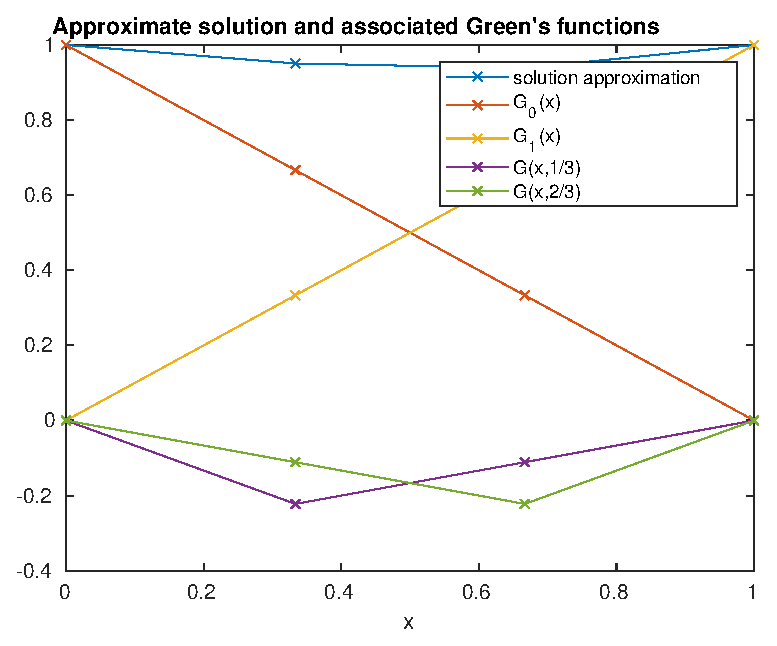
\includegraphics[scale=0.8]{hw2p2.eps}
\end{center}

\section{Problem 3}
Letting
$h = (b-a)/(m+1)$ and $x_j = a + jh$, $j = 0,1, \ldots , m, m+1$, consider the composite trapezoid rule
\[
\int_a^b g(x)\,dx \approx  h \sum_{j=0}^m \frac{g( x_j )+g( x_{j+1} )}{2} 
     =  h \left[ \frac{g( x_0 )}{2} + \sum_{j=1}^m g( x_j ) + 
                   \frac{g( x_{m+1} )}{2} \right] .
\]
\subsection{Part a}
Consider some subinterval $(x_j,x_{j+1})$ where $j\in\{0,\ldots,m\}$. By the fundamental theorem of calculus, we have that 
\[
\int_{x_j}^{x_{j+1}} g(x)\,dx=G(x_{j+1})-G(x_j)
\]
where $G'(x)=g(x)$. Assuming that $g$ (and therefore $G$) is sufficiently smooth, we can Taylor expand around $x=x_j$ (recalling that $x_{j+1}=x_j+h$)
\[
G(x_{j+1})=G(x_j)+hG'(x_j)+\frac{h^2}{2}G''(x_j)+\OO(h^3)=G(x_j)+hg(x_j)+\frac{h^2}{2}g'(x_j)+\OO(h^3).
\]
We can also Taylor expand $g$ around $x=x_j$ as
\[
g(x_{j+1})=g(x_j)+hg'(x_j)+\frac{h^2}{2}g''(x_j)+\OO(h^3).
\]
On this subinterval, the contribution to the composite trapezoid rule is given by \[
\int_{x_j}^{x_{j+1}} g(x)\,dx\approx\frac{h}{2}(g(x_{j})+g(x_{j+1})).
\]
Thus, the error is given by 
\begin{align*}
&\int_{x_j}^{x_{j+1}} g(x)\,dx-\frac{h}{2}(g(x_{j})+g(x_{j+1}))=(G(x_{j+1})-G(x_j))-\frac{h}{2}(g(x_{j})+g(x_{j+1}))\\&=
\left(hg(x_j)+\frac{h^2}{2}g'(x_j)+\OO(h^3)\right)-\frac{h}{2}\left(g(x_{j})+g(x_j)+hg'(x_j)+\frac{h^2}{2}g''(x_j)+\OO(h^3)\right)\\&=
hg(x_j)+\frac{h^2}{2}g'(x_j)+\OO(h^3)-hg(x_j)-\frac{h^2}{2}g'(x_j)-\frac{h^3}{4}g''(x_j)+\OO(h^4)\\&=
\OO(h^3)-\frac{h^3}{4}g''(x_j)+\OO(h^4)=\OO(h^3),
\end{align*}
so we have established that the error on each subinterval is $\OO(h^3)$. Now, we note that the composite trapezoid rule is the sum of the trapezoid rule applied to each subinterval, so its error is the sum of the error on each subinterval. More explicitly, letting $E(j)$ denote the error on the $j$th subinterval $(x_j,x_{j+1})$, the error of the full approximation is given by 
\[
\sum_{j=0}^mE(j)\leq(m+1)\max_{j\in\{0,\ldots,m\}}E(j)=h\OO(h^3)=\OO(h^2),
\]
so the error in the composite trapezoid rule is $\OO(h^2)$.

\subsection{Part b}
Consider 
\[
u(x) = \int_0^1 f( \bar{x} ) G(x; \bar{x} )\,d \bar{x}.
\]
Applying the second form of the composite trapezoid rule above, 
\begin{align*}
u(x)\approx h \left[ \frac{f(x_0)G(x;x_0)}{2} + \sum_{j=1}^m f(x_j)G(x;x_j) + 
                   \frac{f(x_{m+1})G(x;x_{m+1})}{2} \right].
\end{align*}
Now, note that $x_0=0$ and $x_{m+1}=1$, so by the definition of Green's functions (2.31), for any $x\in[0,1]$, $G(x;x_0)=0(x-1)=0$ and $G(x;x_{m+1})=(1-1)x=0$. Thus, 
\[
u(x)\approx h\sum_{j=1}^m f(x_j)G(x;x_j)
\]
is equivalent to the composite trapezoid rule approximation, meaning that it is $\OO(h^2)$ accurate provided that we are able to write the Taylor series as we did in part a. Despite the fact that the $G'(x;x_j)$ has a discontinuity at $x=x_j$, if $f$ is sufficiently smooth, then the derivatives of $f( \bar{x} ) G(x; \bar{x} )$ have a possible discontinuity only at $\bar{x}=x$. In our trapezoid approximation, we consider only $\bar{x}=x_j$ for some $j$, so these potential discontinuities can occur only at gridpoints. Thus, when we do our analysis on a single subinterval, we can simply treat $G$ as linear on that subinterval and proceed with our analysis as before since $f$ is sufficiently smooth. 


\section{Problem 4}
\subsection{Part a}
To find the function
$G(x,\bar x)$ solving
\[
u''(x) = \delta(x-\bar x), \quad u'(0)=0, \quad u(1)=0,
\]
A function that satisfies $u''(x)=0$ has form $u(x)=c_1x+c_2$. so we know that our function must have the form 
\[
G(x,\bar x)=\begin{cases}
c_1x+c_2, \quad 0\leq x\leq\bar{x}\\
d_1x+d_2, \quad \bar{x}\leq x\leq 1.
\end{cases}
\]
Plugging in the BC $u(1)=0$, we conclude that $d_1+d_2=0$. Now, we differentiate $G$
\[
G'(x,\bar x)=\begin{cases}
c_1, \quad 0\leq x\leq\bar{x}\\
d_1, \quad \bar{x}\leq x\leq 1.
\end{cases}
\]
The BC $u'(0)=0$ then gives that $c_1=0$. We also know that the derivative of $G$ must jump by 1 at $x=\bar{x}$, so we conclude that $d_1=c_1+1=1$. This allows us to apply the $d_1+d_2=0$ condition to conclude that $d_2=-1$. Now, we know that $G$ must be piecewise continuous at $x=\bar{x}$, so we equate $c_1\bar{x}+c_2=d_1\bar{x}+d_2$ which becomes $c_2=\bar{x}-1$. Thus, we can conclude that 
\[
G(x,\bar x)=\begin{cases}
\bar{x}-1, \quad 0\leq x\leq\bar{x}\\
x-1, \quad \bar{x}\leq x\leq 1.
\end{cases}
\]
To find the function $G_0(x)$ solving
\[
u''(x) = 0, \quad u'(0)=1, \quad u(1)=0,
\]
we note that $G_0$ must have form $G_0(x)=c_1x+c_2$ and apply the BCs to conclude that $G_0(x)=x-1$. Similarly, we find that the function $G_1(x)$ solving
\[
u''(x) = 0, \quad u'(0)=0, \quad u(1)=1.
\]
is given by $G_1(x)=1$.
\subsection{Part b}
Taking $h=1/3$, $x_0=0, x_1=1/3, x_2=2/3, x_3=1$, we write out the matrix from (2.54)
\[
A=\frac{1}{h^2}\begin{pmatrix}
-h&h&0&0\\
1&-2&1&0\\
0&1&-2&1\\
0&0&0&h^2
\end{pmatrix}=\begin{pmatrix}
-3&3&0&0\\
9&-18&9&0\\
0&9&-18&9\\
0&0&0&1
\end{pmatrix}.
\]
As in problem 2, we let $B$ denote the inverse of $A$ and follow (2.44) through (2.46) to find that
\[
B_{i,0}=G_0(x_i)=x_i-1, \quad i=0,\ldots,3.
\]
\[
B_{i,3}=G_1(x_i)=1, \quad i=0,\ldots,3
\]
and for $j=1,2$,
\[
B_{i,j}=hG(x_i;x_j)=\begin{cases}
h(x_j-1), &i=0,\ldots,j,\\
h(x_i-1), &i=j+1,\ldots,3,\\
\end{cases}
\]
Thus,
\begin{align*}
B&=\begin{pmatrix}
x_0-1&h(x_1-1)&h(x_2-1)&1\\
x_1-1&h(x_1-1)&h(x_2-1)&1\\
x_2-1&h(x_2-1)&h(x_2-1)&1\\
x_3-1&h(x_3-1)&h(x_3-1)&1\end{pmatrix}\\&=
\begin{pmatrix}
-1&(1/3)(-2/3)&(1/3)(-1/3)&1\\
-2/3&(1/3)(-2/3)&(1/3)(-1/3)&1\\
-1/3&(1/3)(-1/3)&(1/3)(-1/3)&1\\
0&0&0&1\end{pmatrix}\\&=
\begin{pmatrix}
-1&-2/9&-1/9&1\\
-2/3&-2/9&-1/9&1\\
-1/3&-1/9&-1/9&1\\
0&0&0&1\end{pmatrix}.
\end{align*}
To confirm that $B=A^{-1}$, we multiply
\[
AB=\begin{pmatrix}
-3&3&0&0\\
9&-18&9&0\\
0&9&-18&9\\
0&0&0&1
\end{pmatrix}\begin{pmatrix}
-1&-2/9&-1/9&1\\
-2/3&-2/9&-1/9&1\\
-1/3&-1/9&-1/9&1\\
0&0&0&1\end{pmatrix}=\begin{pmatrix}
1&0&0&0\\
0&1&0&0\\
0&0&1&0\\
0&0&0&1
\end{pmatrix}=I_4
\]

\section{Problem 5}
For the equation (2.58), the matrix $A^T$ is given by
\[
A^T = \frac{1}{h^2}\begin{pmatrix}
-h & 1 \\
h & -2 & 1 \\
& 1 & -2 & 1 \\
&& \ddots & \ddots & \ddots \\
&&&1&-2&1\\
&&&& 1 & -2 & h \\
&&&&& 1 & -h
\end{pmatrix},
\]
so to find its nullspace, we wish to solve
\[
\frac{1}{h^2}\begin{pmatrix}
-h & 1 \\
h & -2 & 1 \\
& 1 & -2 & 1 \\
&& \ddots & \ddots & \ddots \\
&&&1&-2&1\\
&&&& 1 & -2 & h \\
&&&&& 1 & -h
\end{pmatrix}\begin{pmatrix}
u_0\\ \vdots \\ u_{m+1}
\end{pmatrix}=\begin{pmatrix}
0\\ \vdots \\0
\end{pmatrix}.
\]
Solving the equations in the order that they appear (ignoring the scaling of A since it does not affect things when the RHS is zero), we first need that $-hu_0+u_1=0$, so $u_1=hu_0$. We then have that $hu_0-2u_1+u_2=0$, so $u_2=2u_1-hu_0=hu_0$. We look at the interior inductively, assuming that $u_{j-2}=u_{j-1}=hu_0$ ($j=3,\ldots,m$ where our base case is $u_2=u_1=hu_0$), we have that $u_{j-2}-2u_{j-1}+u_j=0$, so $u_j=2u_{j-1}-u_{j-2}=hu_0$, meaning that $u_j=hu_0$ for $j=3,\ldots,m$. Looking at our penultimate equation, we have that $u_{m-1}-2u_m+hu_{m+1}=0$, so $u_{m+1}=(2u_m-u_{m+1})/h=u_0$. Our last equation $u_m-hu_{m+1}=0$ is clearly satisfied by $u_m=hu_0,u_{m+1}=u_0$. Thus, vectors in the null space of $A^T$ have the form
\[
\begin{pmatrix}
u_0\\hu_0\\ \vdots \\ hu_0\\ u_0
\end{pmatrix}=u_0\begin{pmatrix}
1\\h\\ \vdots \\ h\\ 1
\end{pmatrix},
\]
so the null space of $A^T$ can be represented by 
\[
\text{span}\left\{\begin{pmatrix}
1\\h\\ \vdots \\ h\\ 1
\end{pmatrix}\right\}.
\]
To verify that condition (2.62) must hold for the system to have solutions, recall (as stated above condition (2.62) in the text) that the system $Au=f$ has a solution iff $f$ is orthogonal to the null space of $A^T$. Since we know that $f$ is given by 
\[
\begin{pmatrix}
\sigma_0+\frac{h}{2}f(x_0)\\f(x_1)\\\vdots\\f(x_m)\\-\sigma_1+\frac{h}{2}f(x_{m+1})
\end{pmatrix},
\]
we simply seek to find the conditions for which 
\[
\begin{pmatrix}
\sigma_0+\frac{h}{2}f(x_0)\\f(x_1)\\\vdots\\f(x_m)\\-\sigma_1+\frac{h}{2}f(x_{m+1})
\end{pmatrix}^T\begin{pmatrix}
1\\h\\ \vdots \\ h\\ 1
\end{pmatrix}=0.
\]
We rewrite the LHS to get that 
\[
\sigma_0+\frac{h}{2}f(x_0)+h\sum_{j=1}^mf(x_j)-\sigma_1+\frac{h}{2}f(x_{m+1})=0
\]
which is equivalent to 
\[
\frac{h}{2}f(x_0)+h\sum_{j=1}^mf(x_j)\frac{h}{2}f(x_{m+1})=\sigma_1-\sigma_0
\]
which is precisely condition (2.62).

\section{Problem 6}
\subsection{Part a}
Consider the matrix
\[
A=\frac{1}{h^2} \left( \begin{array}{ccccc}
-h & h  &        &        &      \\
1  & -2 & 1      &        &      \\
   & 1  & \ddots & \ddots &      \\
   &    & \ddots & \ddots & 1    \\
   &    &        & 1      & -2 \end{array} \right)
\]
described as the second method for dealing with Neumann boundary conditions described on page 31 of the text. We wish to find a diagonal matrix $D=\text{diag}(d_0,\ldots,d_m)$ such that $B=DAD^{-1}$ is real symmetric. Note that for $k=0,\ldots,m$, 
\[
B_{k,k+1} = d_{k}A_{k,k+1}/d_{k+1}
\]
and
\[
B_{k+1,k} = d_{k+1}A_{k+1,k}/d_{k}.
\]
Ignoring the factor of $1/h^2$ present since we will equate both sides anyway, since $A_{k,k+1}=A_{k+1,k}$ for $k\geq1$, we can take $d_1=\ldots=d_m=1$ and then $B_{k,k+1}=B_{k+1,k}$ still holds for $k\geq1$. Considering $k=0$, we need that $B_{0,1}=B_{1,0}$, i.e. that 
\[
\frac{d_0}{d_1}h=\frac{d_1}{d_0}.
\]
Plugging in $d_1=1$, we we get that $d_0^2=1/h$, and we choose the positive square root $d_0=1/\sqrt{h}$. Thus, we have that $D=\text{diag}(1/\sqrt{h},1,\ldots,1)$. To confirm the result, we compute 
\begin{align*}
DAD^{-1}&=\begin{pmatrix}
1/\sqrt{h}\\
&1\\
&&\ddots\\
&&&1
\end{pmatrix}\frac{1}{h^2} \left( \begin{array}{ccccc}
-h & h  &        &        &      \\
1  & -2 & 1      &        &      \\
   & 1  & \ddots & \ddots &      \\
   &    & \ddots & \ddots & 1    \\
   &    &        & 1      & -2 \end{array} \right)\begin{pmatrix}
\sqrt{h}\\
&1\\
&&\ddots\\
&&&1
\end{pmatrix}\\&=
\frac{1}{h^2}\left( \begin{array}{ccccc}
-h & \sqrt{h}  &        &        &      \\
\sqrt{h}  & -2 & 1      &        &      \\
   & 1  & \ddots & \ddots &      \\
   &    & \ddots & \ddots & 1    \\
   &    &        & 1      & -2 \end{array} \right).
\end{align*}
This means that $A$ is similar to a symmetric tridiagonal matrix 
via a diagonal similarity transformation

\subsection{Part b}
Now, consider the system (2.57)
\begin{align*}
            \frac{1}{h^2}
            \begin{pmatrix}
                \frac{3h}{2} & -2h & \frac{h}{2} \\
                1 & -2 & 1 \\
                & \ddots & \ddots & \ddots \\
                && 1 & -2 & 1 \\
                &&& 0 & h^2
            \end{pmatrix}
            \begin{pmatrix}
                u_0 \\\vdots \\ u_{m+1}
            \end{pmatrix}
            =
            \begin{pmatrix}
                \sigma \\ f(x_1)\\ \vdots \\ f(x_m) \\ \beta
            \end{pmatrix}.
        \end{align*}
To eliminate the equation on the $0$th row, we note that it has the same nonzero elements as the first row, so we can take a linear combination of them. To elimnate the $u_0$ contribution, multiply the 0th row by $\frac{2}{3h}$ and subtract it from the first row to get the new system
\begin{align*}
            \frac{1}{h^2}
            \begin{pmatrix}
                \frac{3h}{2} & -2h & \frac{h}{2} \\
                0 & -2/3 & 2/3 \\
                & 1 &-2 &1\\
                && \ddots & \ddots & \ddots \\
                &&& 1 & -2 & 1 \\
                &&&& 0 & h^2
            \end{pmatrix}
            \begin{pmatrix}
                u_0 \\\vdots \\ u_{m+1}
            \end{pmatrix}
            =
            \begin{pmatrix}
                \sigma \\ f(x_1)-\frac{2\sigma}{3h}\\ f(x_2)\\ \vdots \\ f(x_m) \\ \beta
            \end{pmatrix}.
        \end{align*}
Now, if we don't care about $u$ at the boundary, we can simply remove the first row from our system since none of our remaining equations depend on $u_0$ (or we can just solve the $0$th equation after solving the remaining system). Similarly, we can remove the last row by plugging in the BC $u_{m+1}=\beta$ to the penultimate equation $\frac{1}{h^2}(u_{m-1}-2u_m+u_{m+1})=f(x_m)$ to get that $\frac{1}{h^2}(u_{m-1}-2u_m)=f(x_m)-\frac{\beta}{h^2}$. Thus, we can write a new system
\begin{align*}
            \frac{1}{h^2}
            \begin{pmatrix}
                -2/3 & 2/3 \\
                1 &-2 &1\\
                & \ddots & \ddots & \ddots \\
                && \ddots & \ddots & 1\\
                &&& 1 & -2 \\
            \end{pmatrix}
            \begin{pmatrix}
                u_1 \\\vdots \\ u_{m}
            \end{pmatrix}
            =
            \begin{pmatrix}
                 f(x_1)-\frac{2\sigma}{3h}\\ f(x_2)\\ \vdots \\ f(x_{m-1}) \\ f(x_m)-\frac{\beta}{h^2}
            \end{pmatrix}
        \end{align*}
which has $m$ equations and $m$ unknowns. Now, we can take 
\[
A=\frac{1}{h^2}
            \begin{pmatrix}
                -2/3 & 2/3 \\
                1 &-2 &1\\
                & \ddots & \ddots & \ddots \\
                && \ddots & \ddots & 1\\
                &&& 1 & -2 \\
            \end{pmatrix}
\]
and show that it is similar to a symmetric tridiagonal matrix 
via a diagonal similarity transformation in the same manner as in part a. Namely, we note that $A_{k,k+1}=A_{k+1,k}$ for $k\geq2$, so we take $d_2=\ldots=d_m=1$. Then, we require that $d_1A_{1,2}/d_2=d_2A_{2,1}/d_1$, i.e. that 
\[
d_1\frac{2}{3}=\frac{1}{d_1}
\]
when we plug in the entries of $A$ and $d_2=1$. Again, we have a quadratic $d_1=\frac{3}{2}$, and we again take the positive square root $d_1=\sqrt{\frac{3}{2}}$ which gives that $D=\text{diag}\left(\sqrt{\frac{3}{2}},1,\ldots,1\right)$. To confirm that this indeed works, we compute
\begin{align*}
DAD^{-1}&=\begin{pmatrix}
\sqrt{\frac{3}{2}}\\
&1\\
&&\ddots\\
&&&1
\end{pmatrix}\frac{1}{h^2}
            \begin{pmatrix}
                -2/3 & 2/3 \\
                1 &-2 &1\\
                & \ddots & \ddots & \ddots \\
                && \ddots & \ddots & 1\\
                &&& 1 & -2 \\
            \end{pmatrix}
\begin{pmatrix}
\sqrt{\frac{2}{3}}\\
&1\\
&&\ddots\\
&&&1
\end{pmatrix}\\&=
\frac{1}{h^2}
            \begin{pmatrix}
                -2/3 & \sqrt{\frac{2}{3}} \\
                \sqrt{\frac{2}{3}} &-2 &1\\
                & 1 & \ddots & \ddots \\
                && \ddots & \ddots & 1\\
                &&& 1 & -2 \\
            \end{pmatrix}.
\end{align*}
\end{document} 
